\subsection{Numerical evaluation of }

\begin{figure}[!htbp]
    \centering
    \subfloat[\label{fig-power-4cycle-chisq}]{
        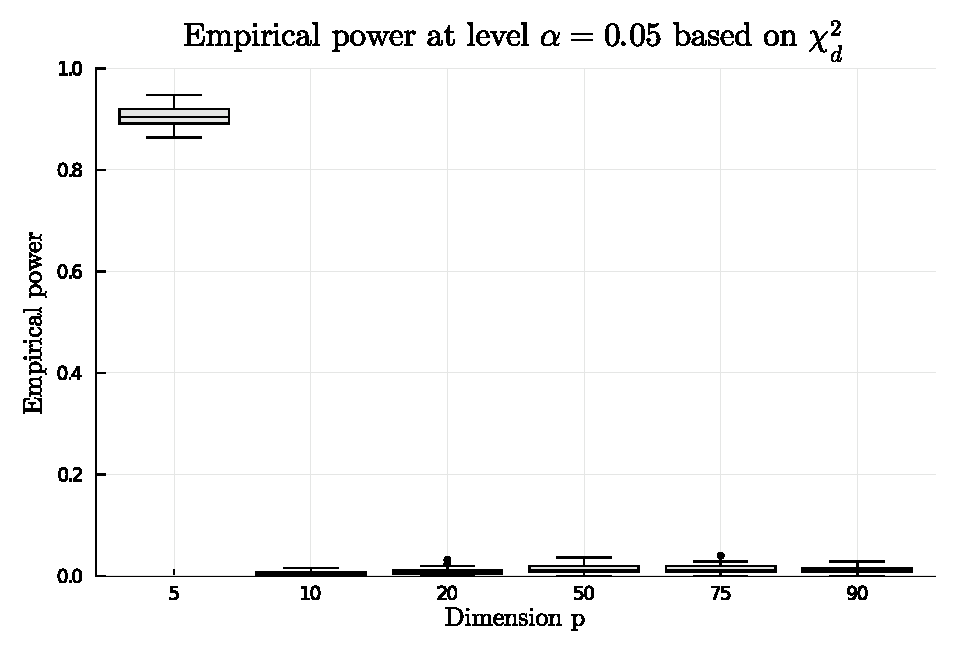
\includegraphics[width=7cm]{power_complete_to_chordless4cycle_chisq.eps}
    }
    \subfloat[\label{fig-power-4cycle-beta}]{
        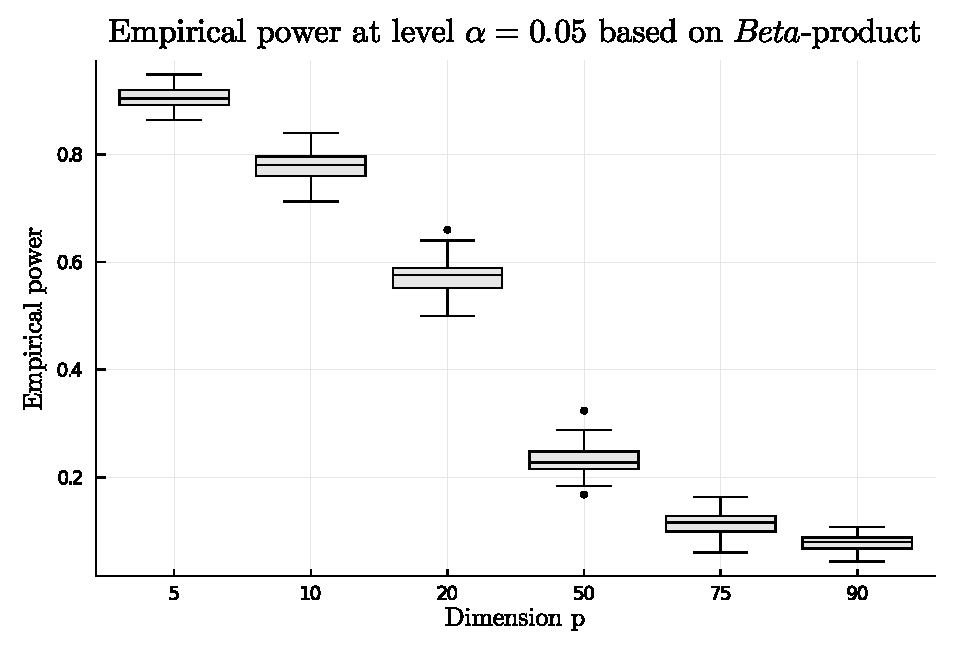
\includegraphics[width=7cm]{power_complete_to_chordless4cycle_beta.eps}
    }
\end{figure}

\begin{figure}[!htbp]
    \centering
    \subfloat[\label{fig-size-cycle-chisq}]{
        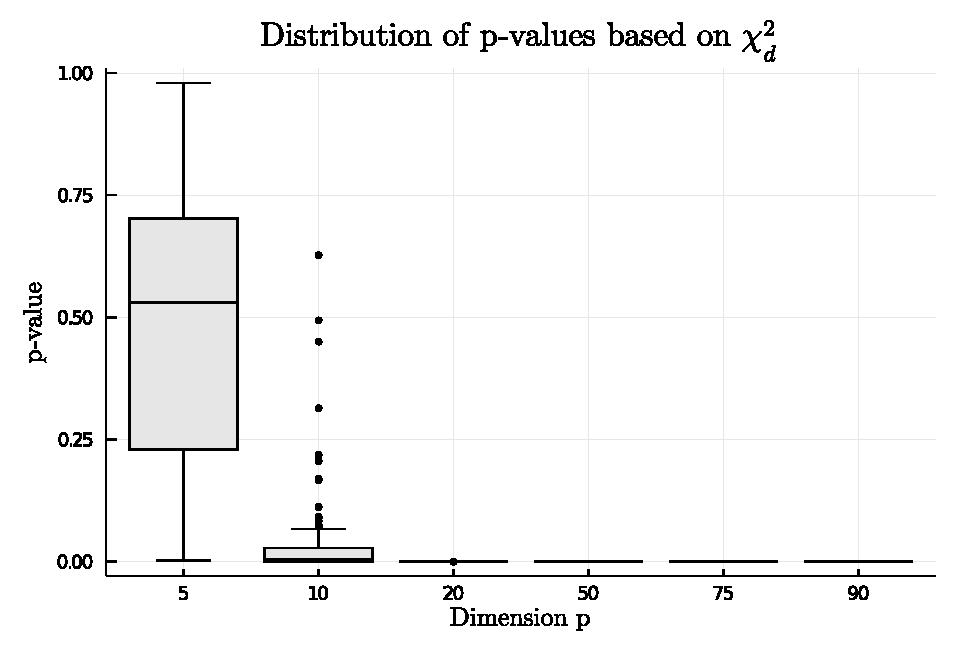
\includegraphics[width=7cm]{complete_to_pcycle_chisq.eps}
    }
    \subfloat[\label{fig-size-cycle-beta}]{
        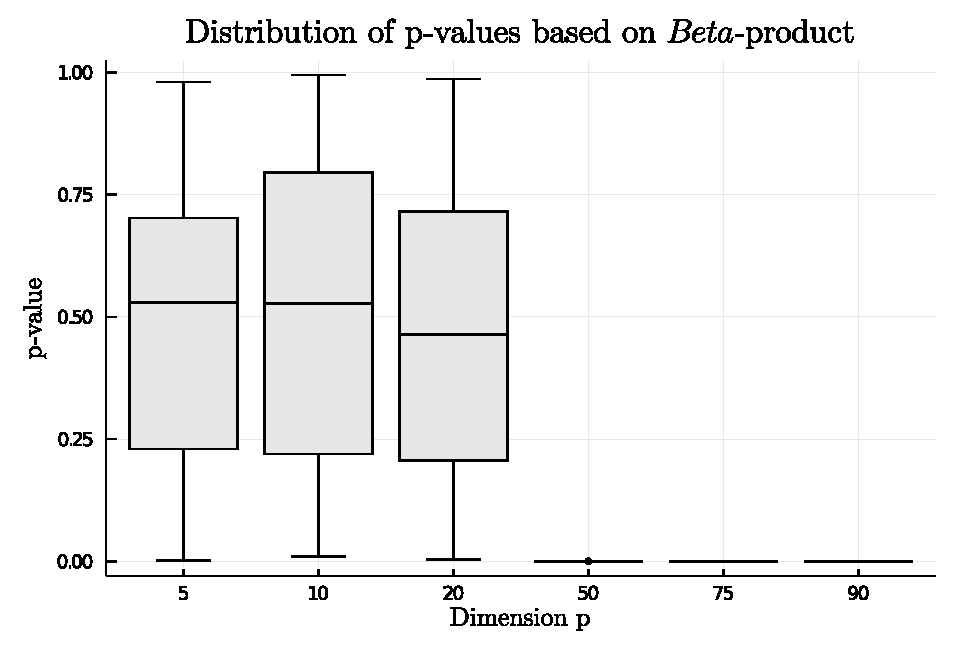
\includegraphics[width=7cm]{complete_to_pcycle_beta.eps}
    }
\end{figure}

\begin{figure}[!htbp]
    \centering
    \subfloat[\label{fig-power-cycle-chisq}]{
        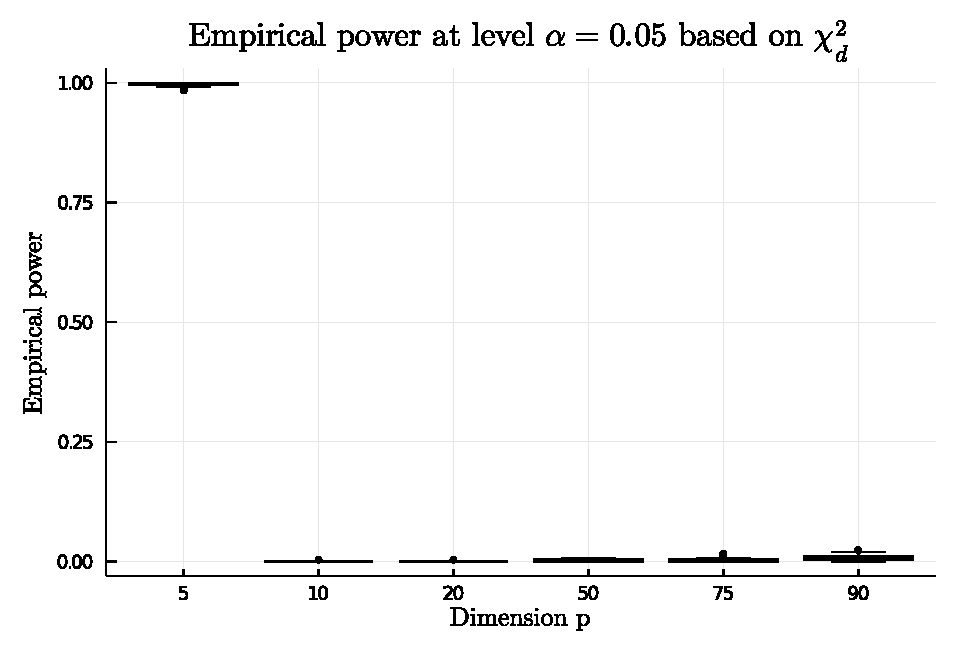
\includegraphics[width=7cm]{power_complete_to_cycle_chisq.eps}
    }
    \subfloat[\label{fig-power-cycle-beta}]{
        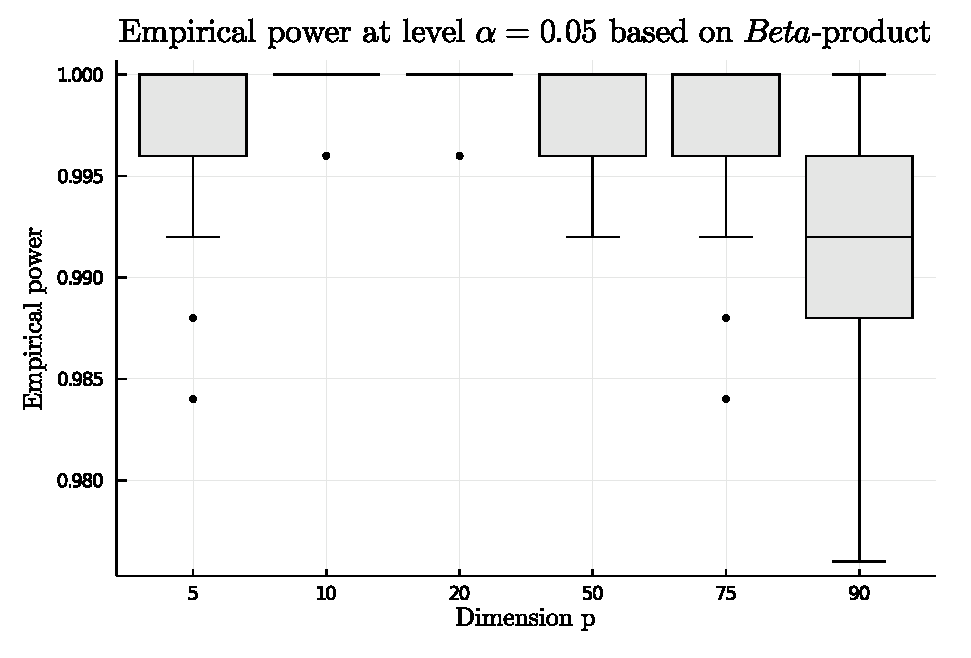
\includegraphics[width=7cm]{power_complete_to_cycle_beta.eps}
    }
\end{figure}


We now compare different properties of the hypothesis test based on the $\chi^2_d$ approximation to the likelihood ratio and the product of Beta distributions described in \note{todo ref}. We are interested in evaluating the size and power of the tests resulting from these two asymptotic approximations. The \textit{size} of a test is its probability of rejecting the null hypothesis when it is true, also called \textit{type I error}. The \textit{power} of a test is its probability to reject the null hypothesis when it is false. One is interested in tests maximizing power while keeping the proba bility of doing a type I error under a pre-defined level $\alpha$. In other words, a good test maximizes the probability of discovering true phenomena while keeping the probability of making a false discovery under control. 

We now present experiments aiming at exploring the size and power of the statistical tests constructed based on the $\chi^2_d$ approximation to the distribution of the $\Lambda(S_n)$ statistic and the product of Betas approximation to the distribution of the $Q(S_n)$ statistic. In particular, we are interested in evaluating how the different tests behave when the sample size is kept fix and the number of parameters increases.

In the first setup, we consider a sequence of problems in which the number of nodes in the graph $\G$ grows while the number of edges removed to form $\G_0$ is kept fix. In particular, we will consider the complete graph $\G = ([p], E)$ with $E = \eset{\eset{i, j} : i, j \in [p], i \neq j}$ and the subgraph $\G_0 = ([p], E_0)$ with $E_0 = E \setminus \eset{\eset{1, 3}, \eset{2, 4}}$. As shown in Figure \ref{fig-graph-exp-1}, the subgraph $\G_0$ can be decomposed in the cycle $\eset{1, 2, 3, 4}$ and the clique $C_p = [p] \ \eset{1,2,3,4}$ formed with the rest of the nodes, such that each nodes of the cycle forms a clique when added to $C$. In $\G_0$, the largest clique is $C \cup \eset{i}$ for $i \in \eset{1, 2, 3, 4}$ which has a size of $p - 3$. The minimal chordal cover of $\G_0$ can be constructed by adding back the edge $\eset{1, 3}$ or $\eset{2, 4}$ to break to cycle. If we consider the chordal cover constructed by additing the edge $e = \eset{1, 2}$, the maximal clique is $C \cup \eset{1, 2, 4}$ which contains $p - 1$ nodes. Hence, from (\ref{eq-mlt-bounds}), the maximum likelihood threshold $\G_0$ satisfies
\begin{equation*}
    p - 3 \leq \t{mlt}(\G_0) \leq p - 2,
\end{equation*}
and the maximum likelihood estimator of $\Omega$ under $\G_0$ exists almnost surely if $n \geq p - 2$.

In this setup, the quantities of interest are the entries of the precision matrix corresponding to the 2 edges removed from $\G$ to construct $\G_0$, $\Omega_{13}$ and $\Omega_{24}$, we call \textit{nuisance parameters} the other entries of $\Omega$ which are not tested in the model comparison. Hence, in this setup, the number of parameters of interest corresponding to the constraints encoded in $\G_0$ is fix while the number of nuisance parameters grows quadratically with $p$.  In this hypothesis test, $d = |E| - |E_0| = 2$ and hence the likelihood ratio statistic $\Lambda(S_n)$ asymptotically follows a $\chi^2_2$ distribution. Following the procedure described in the previous section, the $Q(S_n)$ statistic is asymptotically distributed as the product of two independent Beta distributed random variables $B((n - f(\eset{1,3}) - 1), 1/2)$ and $B((n - f(\eset{2,4}) - 1), 1/2)$. Regardless of the order in which the edges are removed $f(\eset{2,4}) = f(\eset{1, 3}) = p - 2$ and hence $Q(S_n)$ is asymptotically distributed as $B((n-p+1)/2, 1/2)B((n-p+1)/2, 1/2)$.

\begin{figure}[tbp!]
    \centering
    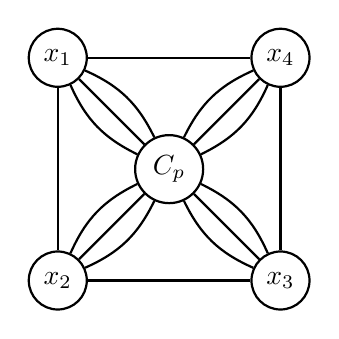
\begin{tikzpicture}[node distance={20mm}, thick, main/.style = {draw, circle}] 
        \node[main] (C) {$C_p$};
        \node[main] (1) [above left of=C] {$x_1$}; 
        \node[main] (2) [below left  of=C] {$x_2$};
        \node[main] (3) [below right of=C] {$x_3$}; 
        \node[main] (4) [above right of=C] {$x_4$};
        \draw (1) -- (2);
        \draw (2) -- (3);
        \draw (4) -- (3);
        \draw (1) -- (4);
        
        \draw (1) -- (C);
        \path[-] (1) edge [bend left=20] node {} (C);
        \path[-] (1) edge [bend right=20] node {} (C);

        \draw (2) -- (C);
        \path[-] (2) edge [bend left=20] node {} (C);
        \path[-] (2) edge [bend right=20] node {} (C);
        
        \draw (3) -- (C);
        \path[-] (3) edge [bend left=20] node {} (C);
        \path[-] (3) edge [bend right=20] node {} (C);

        \draw (4) -- (C);
        \path[-] (4) edge [bend left=20] node {} (C);
        \path[-] (4) edge [bend right=20] node {} (C);
    \end{tikzpicture}
    \caption{The graph $\G_0$ depicted here is a subgraph of the complete graph $\G$ which encodes a constant number of independence constraints as $p$ grows.}
    \label{fig-graph-exp-1}
\end{figure}

To evaluate the size of each approximation, we follow the numerical procedure used in Tang et al.\,\cite{Tang2020}. For each value of $p = 5, 10, 20, 50, 75, 90$, we perform a series of experiments with the goal of evaluting the approximations of the respective test statistics under the null hypothesis. Each each experiment, the dimension $p$ is fixed, as well as the sample size $n = 100$. Then, a random precision matrix $\Omega \in \S(\G_0)$ is sampled as described in \note{todo} and a sample $X_1, \ldots, X_n \simiid N_p(0, \Omega^{-1})$ is used to compute the statistics $\Lambda(S_n)$ and $Q(S_n)$. We perform $N = 25000$ experiments to create a sample two large samples of $\Lambda(S_n)$ and $Q(S_n)$ and compute for each test statistic the p-value resulting from the associated approximation, giving for each test $N = 25000$ p-values. Under the null hypothesis, the approximate distributions are asymptotically valid and hence the p-values are asymptotically uniform on $[0, 1]$. As shown in Figure \ref{fig-complete-to-4cycle}, the distribution of the p-values in the likelihood ratio test is not uniform for $p \geq 10$ while appear to remain uniform in the test based on the $Q(S_n)$ statistic even for $p$ approaching $n$.

\begin{figure}[!tbp]
    \centering
    \subfloat{
        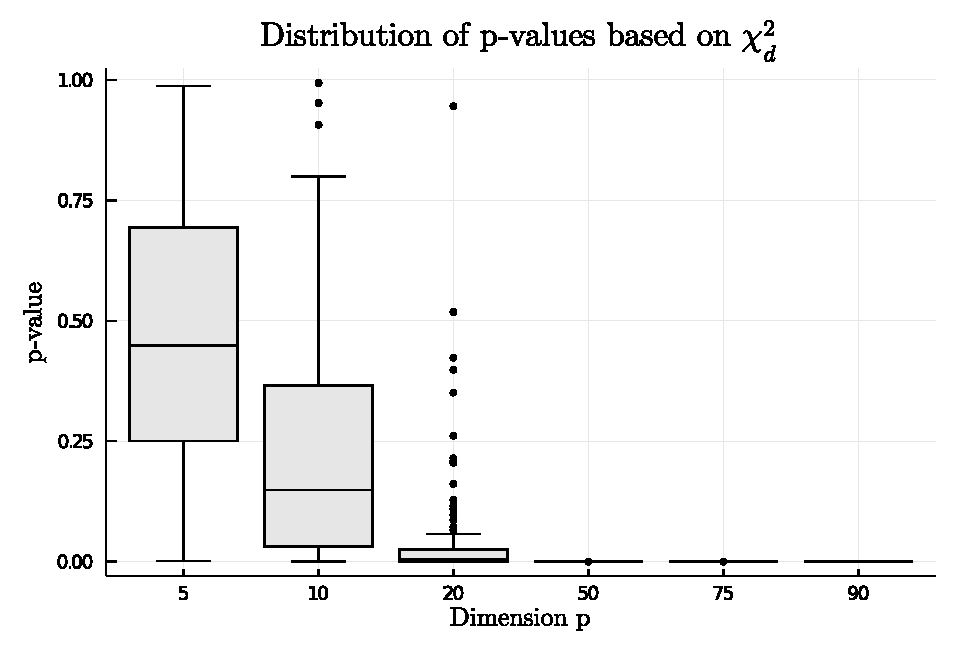
\includegraphics[width=7cm]{complete_to_chordless4cycle_chisq.eps}
    }
    \subfloat{
        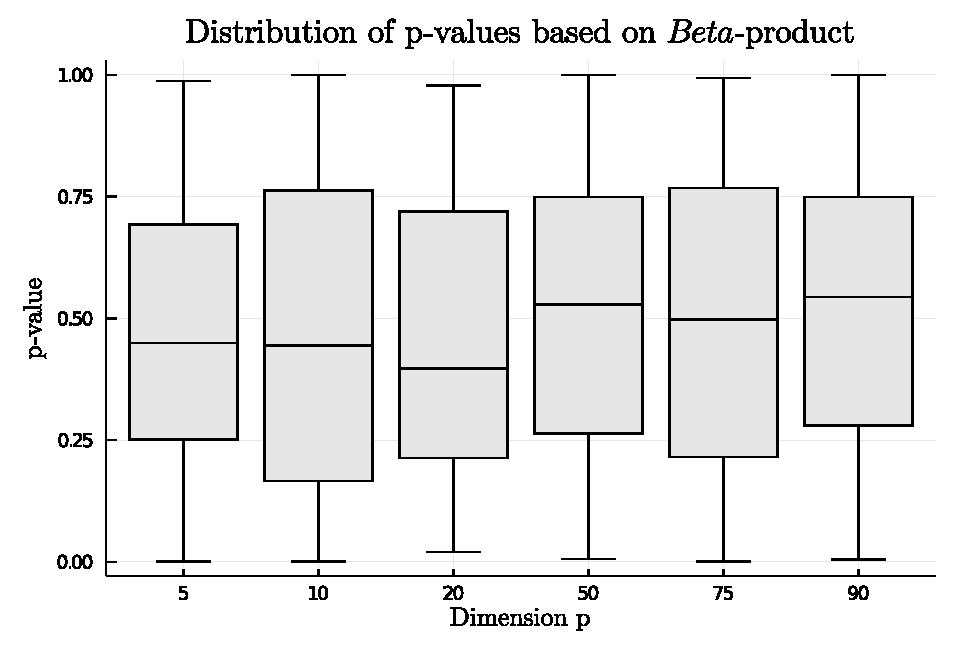
\includegraphics[width=7cm]{complete_to_chordless4cycle_beta.eps}
    }
    \caption{Distribution of the p-values computed from the $\chi^2_d$ and product of Betas approximations for $n = 100$ and $p = 5, 10, 20, 50, 75, 90$. The $\chi^2_d$-based test appears to fail for $p \geq 10$ while the product of Betas test seems to hold and be exact for $p$ approaching $n$.}
    \label{fig-complete-to-4cycle}
\end{figure}

To evaluate the power of each approximation, we estimate the empirical rejection rate under the alternative hypothesis given a fix nominal level $\alpha = 0.05$. Similarly to the evaluation of the size of each test, we perform for different values of $p = 5, 10, 20, 50, 75, 90$ a series of experiments aiming at estimating the average power of each test for a fix $n = 100$. In each experiment, we generate a random precision matrix $\Omega \in \S(\G)$ as described in \note{todo} and repeat the same experiment as in the evaluation of the size of the tests. 